\documentclass[a4paper]{article}
\usepackage[margin=20mm]{geometry}
\usepackage{amsmath,graphicx,booktabs}
\usepackage[hidelinks]{hyperref}

\title{Classical and Quantum-Assisted Search for QOBLIB Network Design}
\author{Quantum Icing Team}
\date{}

\begin{document}
\maketitle

\begin{abstract}
We combine parallel tempering and iterated local search on the QOBLIB \texttt{network24} instance, scoring each topology
by solving a continuous routing problem. A first parallel tempering run supplied a solution of 670,621.
Iterated local search reduced the objective to 661,760, and a second parallel tempering run reduced it to 657,121
in 62 seconds from that warm start. The verified integer objective is 0.989\% below the published reference of 663,688.
We then derive smaller instances by deleting vertices from the incumbent and refine them with LP-scored local search
and compound moves sampled by simulated QAOA, continuing the chain down to \texttt{network06}.
A final campaign ranks degree-preserving rewires by a congestion estimate and selects them with simulated Grover sampling.
It lowers \texttt{network19}, \texttt{network20}, \texttt{network22} and \texttt{network23} further.
All seven instances from \texttt{network18} to \texttt{network24} now beat their published references, by 0.924\% to 4.102\%.
The largest reduction is \texttt{network23}, at 632,319.
Exhaustive enumeration proves \texttt{network05} and \texttt{network06} optimal. We match the proven optima of
\texttt{network07}--\texttt{network09} and the reference value of \texttt{network12}.
\end{abstract}

\section{Problem formulation}

A QOBLIB network design instance specifies traffic demands \(d_{sv}\) from source \(s\) to destination \(v\).
A topology is a set \(A\) of directed arcs, with two incoming and two outgoing arcs at each of the \(n\) vertices.
The \(n(n-1)\) binary link decisions therefore select exactly \(2n\) arcs. The objective is to minimize the largest arc load.

For fixed \(A\), let \(f^s_{uv}\) be the amount of traffic from source \(s\) carried by arc \((u,v)\).
Demands are scaled by 1,000 to match the benchmark's units. The routing relaxation is
\begin{equation}
\label{eq:routing}
\begin{aligned}
z_{\mathrm{LP}}(A) = \min_{f,z}\;& z\\
\text{subject to}\quad
\sum_{u:(u,v)\in A} f^s_{uv} - \sum_{w:(v,w)\in A} f^s_{vw}
  &= 1{,}000\,d_{sv} && (s,\ v\ne s),\\
\sum_s f^s_{uv} &\le z && ((u,v)\in A),\\
f^s_{us}&=0 && ((u,s)\in A),\\
f^s_{uv}&\ge 0 && (s,\ (u,v)\in A).
\end{aligned}
\end{equation}
We solve \eqref{eq:routing} with HiGHS and use \(E(A)=z_{\mathrm{LP}}(A)\) as the search energy.
The benchmark requires integer flows, which we compute when a topology can improve the incumbent.

\section{Search methods for \texttt{network24}}

\subsection{Parallel tempering}

Parallel tempering~\cite{hukushima1996} runs several replicas at fixed temperatures.
Each replica uses the Metropolis acceptance probability \(\min\{1,\exp[-(E'-E)/T]\}\) for a proposed change from \(E\) to \(E'\).
A high-temperature replica can more readily accept increases in congestion and leave a local minimum.
Exchanging configurations gives a low-temperature replica access to the topologies explored at higher temperatures.
The exchange probability for neighboring slots \(i,j\) is
\[
 p_{\mathrm{exchange}}=\min\!\left\{1,\exp\!\left[
 (T_i^{-1}-T_j^{-1})(E_i-E_j)\right]\right\}.
\]
Each round consists of 15 local steps followed by exchange attempts, alternating between the odd and even adjacent pairs.

A two-arc exchange replaces \((a,b),(c,d)\) with \((a,d),(c,b)\), preserving all degrees. We also rotate the heads
of three arcs and reverse directed triangles. The probabilities of drawing these move types were
77\%, 20\%, and 3\%, respectively, before rejection of self-loops and duplicate arcs. For exchanges and rotations,
half the draws for the first arc are uniform and half are weighted by the capacity duals from \eqref{eq:routing}.
Larger duals indicate arcs whose extra capacity would reduce the objective locally.

Solving a routing LP for every candidate would be expensive, so we first rank candidates by a bound on congestion.
Let \(h_A(s,v)\) be the directed shortest-path distance in hops. Every unit of demand from \(s\) to \(v\) contributes
at least \(h_A(s,v)\) units to the sum of arc loads. That sum is at most \(\lvert A\rvert z\), giving
\begin{equation}
\label{eq:bound}
 L(A)=\frac{1{,}000}{\lvert A\rvert}\sum_{s,v}d_{sv}\,h_A(s,v)\le z_{\mathrm{LP}}(A).
\end{equation}
Each step draws up to 60 candidates, with a 50\% probability of attempting a second move per candidate.
We retain the candidate with the smallest bound, skipping those with a cached LP value above \(E+3T\).
To implement the Metropolis test we draw \(U\) uniformly from \((0,1)\), which gives the acceptance threshold \(E-T\log U\).
If the bound \eqref{eq:bound} exceeds that threshold, the candidate is rejected.
Otherwise we use its cached LP value or solve \eqref{eq:routing}.
The biased proposal and Metropolis rule are used without a Hastings correction, yielding an optimization heuristic.

\subsection{Iterated local search}

Iterated local search (ILS) alternates a perturbation of the current topology with descent to a local minimum~\cite{lourenco}.
Our descent uses two-arc exchanges, reversals of directed cycles of length three or four, and swaps of two vertex labels.
For the label swap \(\pi\), each arc \((u,v)\) becomes \((\pi(u),\pi(v))\). The demand matrix stays fixed, so an unchanged
graph structure can yield a different routing objective.

Descent ranks the neighbors by a weighted version of \eqref{eq:bound}, replacing hop counts by weighted distances and
\(\lvert A\rvert\) by the sum of the arc weights. It takes the first LP improvement and repeats.
To reduce solve time, ILS updates the routing LP in place and reuses the simplex basis of the parent topology.
Once descent stalls, perturbations of two to eight moves provide new starting points for descent.

The run also used an initial look-ahead from the shared starting topology. It scored neighbors within 1.5\% of the
starting objective, divided the ranked list among five chains, and ran descent from up to 12 such neighbors per chain.
This lets descent reach a lower objective by first visiting a neighbor with higher congestion.

\section{Computational results for \texttt{network24}}

\begin{table}[htbp]
\centering
\caption{Checked objectives along the search that produced the submission. Times are measured from each run's start.}
\label{tab:runs}
\begin{tabular}{@{}lrrrr@{}}
\toprule
Run & Starting objective & Handoff or submission & Decrease & Time (s)\\
\midrule
PT r6    & 673,253 & 670,621 & 2,632 & 1,211\\
ILS run8 & 670,621 & 661,760 & 8,861 &   110\\
PT r7    & 661,760 & 657,121 & 4,639 &    62\\
\bottomrule
\end{tabular}
\end{table}

Table~\ref{tab:runs} and Figure~\ref{fig:progress} follow the topology passed from one run to the next.
The two PT runs used ten workers and ten geometrically spaced temperatures from 450 to 2,500. In each run the two
coldest slots started from the incumbent and the other eight from random routable topologies.

\begin{figure}[htbp]
\centering
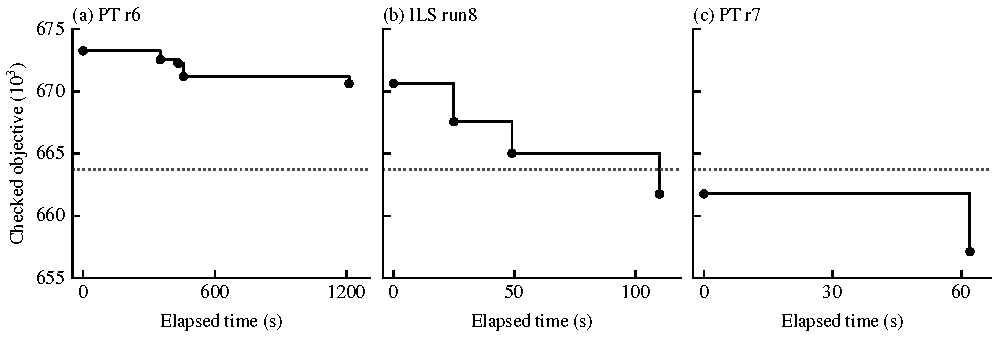
\includegraphics[width=\linewidth]{figures/pt-progress.pdf}
\caption{Checked objective along the PT--ILS--PT sequence. Each panel has its own time origin and ends at the
incumbent passed to the next stage or submitted. The dotted line is the QOBLIB reference.}
\label{fig:progress}
\end{figure}

\newpage
Run r6 inherited the checked 673,253 topology from a preliminary PT run, r5, which started at 674,907.
Run r6 used seed 7 and a 30-minute budget. ILS took the 670,621 incumbent found at round 595,
while r6 was still running. All five ILS chains started from that topology and ran with a 20-minute budget.
During the initial look-ahead, the chain with seed 702 reached checked objectives of 667,560, 665,040, and 661,760.
A vertex-label swap during descent produced the last improvement, the first in this sequence below the QOBLIB reference
of 663,688~\cite{qoblib}.

The second PT run, r7, used seed 8 and a 20-minute budget, starting from the ILS incumbent of 661,760.
In round 30, after 62 seconds, the coldest slot produced the submitted objective of 657,121, an improvement of
4,639 (0.701\%) from the ILS warm start and 6,567 (0.989\%) from the QOBLIB reference.
The incumbent stayed at 657,121 through round 597, when the run ended.

The local acceptance rate increased from 0.8\% at \(T=450\) to 33.8\% at \(T=2500\) (Figure~\ref{fig:diagnostics}).
The 544--659 pair accepted 2.7\% of its exchange attempts, while the 450--544 pair accepted 86.6\%.
The low acceptance across 544--659 indicates a bottleneck on this temperature ladder.

\begin{figure}[htbp]
\centering
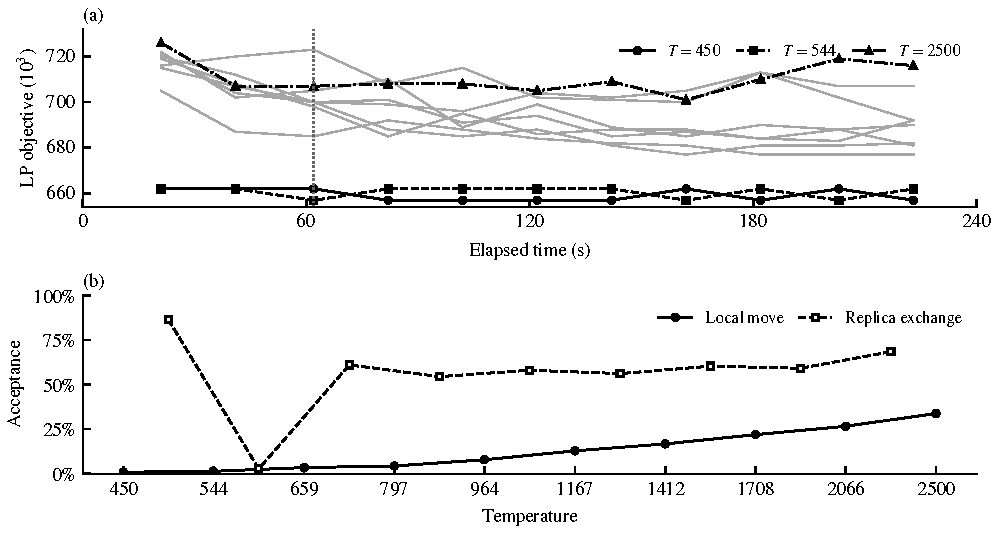
\includegraphics[width=\linewidth]{figures/pt-diagnostics.pdf}
\caption{Search dynamics in r7. (a) LP objective by temperature slot, sampled every ten rounds after exchanges and
rounded to the nearest thousand. The dotted line marks the verified improvement. (b) Cumulative acceptance rates
at round 597. Exchange rates are plotted at the geometric mean of each temperature pair.}
\label{fig:diagnostics}
\end{figure}

% \section{Verification and reproducibility}

% We re-solve \eqref{eq:routing} with integer variables when a candidate's LP bound permits an improvement.
% The referee checks the resulting \texttt{.sol} file before it replaces the incumbent.
% For the submitted topology, the LP gives \(657{,}120.967742\), so the verified maximum load of \(657{,}121\) is
% optimal for that topology. All computations were classical and used zero qubits.

% Verify the submitted file from the repository root with the Python environment active.
% \begin{verbatim}
% NETWORK_SOL_DIR=deliverables/network24 \
%   python network_pipeline.py status
% \end{verbatim}

% The traces come from \path{pt_r6.log}, \path{ils_run8.out}, and \path{pt_r7.log} under \path{ai_context/logs/}.
% The final topology is stored in \path{solutions/agent_pt/r7_best24.json}.
% The repository's \path{deliverables/README.md} gives the stage commands. Replaying the ILS and final PT stages
% from their historical starts would require recovering or regenerating the 670,621 and 661,760 topologies.

\clearpage
\section{Compound-move search for smaller instances}

\subsection{Warm starts by vertex deletion}

The demand matrix for \texttt{network}\(n\) is the leading \(n\times n\) block of the same benchmark matrix.
To construct a warm start, we delete vertex \(n+1\) from the incumbent on \texttt{network}\(n+1\).
If \(a,b\) are its predecessors and \(c,d\) its successors, we try the two reconnections
\(\{(a,c),(b,d)\}\) and \(\{(a,d),(b,c)\}\). Both restore the degree counts.
We score the valid reconnections by routing LP and keep the lower one. If both reconnections create self-loops
or duplicate arcs, we repair the degrees before scoring.
Deleting the last vertex of the submitted \texttt{network24} topology gives a score of 642,084 for \texttt{network23},
already 2.621\% below its reference. After each search, we use its best topology to initialize the next smaller instance.

\subsection{QUBO over degree-preserving moves}

Starting from the derived topology, we perform first-improvement descent over valid two-arc exchanges in
random order. The routing LP is updated in place and initialized with the parent simplex basis.
When a full pass finds no improving exchange, we retain up to \(N=18\) exchanges with the smallest LP increases
among neighbors within 2\% of the current congestion.

Let \(z\) be the current LP objective, \(z_i\) the objective after exchange \(i\), and \(z_{ij}\) the objective after
applying both exchanges \(i,j\). We compute \(d_i=z_i-z\) and solve the routing LP for every compatible pair to obtain
\[
J_{ij}=z_{ij}-z-d_i-d_j .
\]
An exchange pair conflicts if it shares an original arc or its combined update is invalid. For binary flags
\(y_i\) indicating which exchanges to apply, and conflict set \(\mathcal C\), the sampled QUBO is
\begin{equation}
\label{eq:compound}
E(y)=\frac{1}{s_0}\left[\sum_i(d_i-\mu)y_i
       +\sum_{\substack{i<j\\(i,j)\notin\mathcal C}}J_{ij}y_iy_j\right]
      +P\sum_{(i,j)\in\mathcal C}y_iy_j .
\end{equation}
Here \(s_0=\max(1,\operatorname{median}_i|d_i|)\), \(\mu\) is the fourth-smallest retained \(d_i\)
(or the last if fewer are retained), and \(P=1+2(\max_i|d_i-\mu|+\max_{ij}|J_{ij}|)/s_0\),
with the second maximum taken as zero if there are no compatible pairs.
Negative \(J_{ij}\) identifies a pair whose joint cost is smaller than the sum of its individual costs.
The pair evaluations give exact LP changes for two compatible exchanges. For three or more moves,
the quadratic expression approximates the routing objective.

\subsection{Sampling and acceptance}

We use Divi 0.16.2 to run two-layer QAOA~\cite{farhi2014} on the local Maestro statevector simulator.
One qubit represents each shortlisted exchange. The winning process used at most 18 qubits,
4,000 shots per circuit, and a Monte Carlo optimizer with population 16 and eight iterations.
We keep unique samples with at least two moves and no flagged conflicts, then test up to 30 of the lowest-energy
samples for validity and evaluate their actual congestion by LP. The pair scan supplies a classical proposal from the same shortlist.

An improving exact pair takes precedence if its LP objective is more than 0.5 units lower than the best sampled compound.
Otherwise an improving sample is accepted. A sample within 1.5\% of the current congestion can seed the next descent
as a perturbation. The fallback is a random two- or three-exchange perturbation. Every fourth cycle restarts from the best topology.

\clearpage
\section{Trace of the \texttt{network23}--\texttt{network18} chain}

The winning process, p1, used seed 1. It searched instances in descending order from 23 to 18, with budgets
of 2.5, 4.5, 4.5, 4.5, 4.5, and 6 minutes, respectively. Table~\ref{tab:hybrid-trace} gives the verified
endpoints and the elapsed time at which the corresponding topology first appeared in the search log.

\begin{table}[htbp]
\centering
\caption{Warm starts and origins of the delivered solutions. Discovery time is measured from each instance's logged start.
Integer routing and checking sometimes occurred later.}
\label{tab:hybrid-trace}
\begin{tabular}{@{}lrrrl@{}}
\toprule
Instance & Warm start & Checked & Time (s) & Step producing the topology \\
\midrule
\texttt{network23} & 642,084 & 639,739 & 28 & Initial descent \\
\texttt{network22} & 610,880 & 606,424 & 74 & Descent after QAOA pair \\
\texttt{network21} & 573,625 & 562,362 & 65 & Exact pair scan \\
\texttt{network20} & 529,967 & 519,343 & 88 & Descent after QAOA perturbation \\
\texttt{network19} & 502,600 & 488,895 & 71 & Pair scan and descent after QAOA \\
\texttt{network18} & 481,400 & 473,000 &  8 & Initial descent \\
\bottomrule
\end{tabular}
\end{table}

\begin{figure}[htbp]
\centering
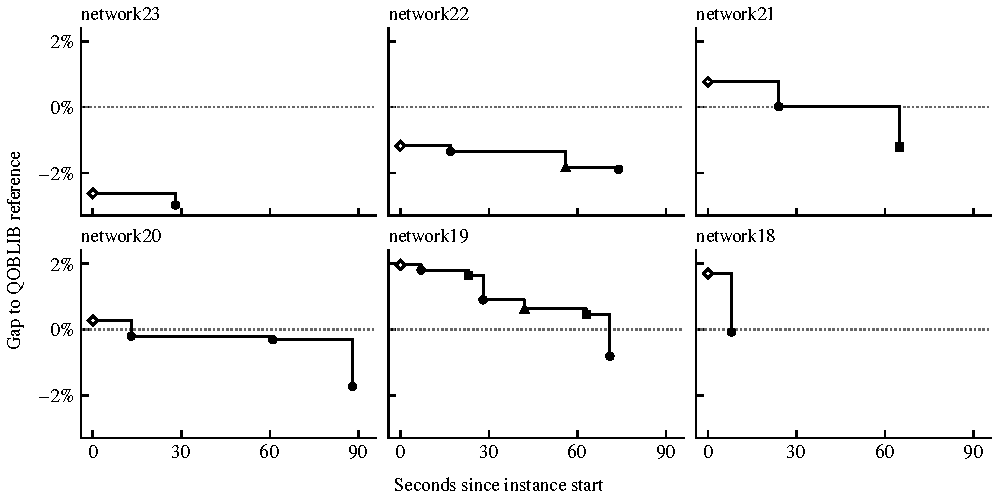
\includegraphics[width=\linewidth]{figures/chain-progress.pdf}
\caption{Logged incumbent routing-LP objectives during p1, relative to each instance's reference.
Open diamonds mark the derived starts, circles mark descent, squares mark exact pairs, and triangles mark
improving QAOA proposals. Traces end at discovery of the delivered topology.}
\label{fig:chain}
\end{figure}

The \texttt{network23} result was found before its first QAOA call. The chain's largest improvement over the
published reference, 2.977\%, therefore comes from the classical warm start and descent.
For \texttt{network22}, QAOA returned a two-move compound at 606,829, the same objective as the exact best pair.
Descent from that topology reached the submitted 606,424. The final \texttt{network21} and \texttt{network18}
topologies came from the pair scan and from descent, respectively, with warm starts inherited from the hybrid chain.

On \texttt{network20}, the sampled perturbation temporarily raised the LP objective from about 526,873 to 532,187.
The next descent lowered it to 519,343. On \texttt{network19}, QAOA found four compatible moves with an LP
objective of 496,000, compared with 497,143 for the best pair at the same topology. An exact pair accepted
from the new topology and a subsequent descent reached 488,895 (Figure~\ref{fig:chain}).

\clearpage
\section{Extensions after the first hand-in}

\subsection{The deletion chain below \texttt{network18}}

The vertex-deletion chain of the previous section was continued from \texttt{network18} down to \texttt{network06},
with the same descent, exact pair scans and QAOA compound proposals. Later runs improved \texttt{network18} from 473,000 to 469,000
and \texttt{network20} from 519,343 to 518,305, and an independent run lowered \texttt{network22} from 606,424 to 604,540.
Below \texttt{network18} the chain reaches the proven optimum of \texttt{network08} (170,231) and the reference value of
\texttt{network12} (276,474). On \texttt{network10}--\texttt{network17} it remains 0.53--2.03\% above the references,
which come from a parallel-tempering submission.

\subsection{Rewire search with simulated Grover sampling}

The final campaign starts from the seven hand-in topologies \texttt{network18}--\texttt{network24}.
Each round generates valid rewires by shuffling the heads of two to six arcs, which preserves all degrees.
It shortlists candidates by demand-weighted path lengths and excess loads, starting from tolls given by the routing LP duals.
Over the shortlist indices it prepares a uniform superposition, and a phase oracle marks roughly the best 12\% under the estimate.
Grover reflections~\cite{grover} amplify the marked indices. The simulation uses at most 11 index qubits and 2,048 shots per round.
Up to 120 distinct measured topologies are scored exactly by \eqref{eq:routing}. The walk accepts bounded uphill steps and restarts
from its best topology. A separate Qiskit circuit reproduced the probabilities of the first improving \texttt{network23} round
to within \(1.3\cdot10^{-13}\).

The campaign improved \texttt{network19} to 486,579, \texttt{network20} to 516,397, \texttt{network22} to 604,229 and
\texttt{network23} to 632,319, a further 7,420 below the hand-in. At an equal routing budget with the same shortlists,
Grover selection beat uniform selection in 294 rounds and lost 14 (56 ties).
Greedy selection by the congestion estimate tied in 309 rounds and won 51 of the remaining 55.
It matched the routing score in every round that set a new record. The improvement therefore comes from the
classically computed estimate, with Grover sampling as a valid way to concentrate on its marked candidates.

\subsection{Exact enumeration and LP-dual tabu search}

Every node chooses two distinct successors, so all \(\binom{n-1}{2}^n\) choices can be enumerated, keeping those
with in-degree two and scoring each by \eqref{eq:routing}. This proves \texttt{network05} (216 valid topologies) and
\texttt{network06} (7,570 topologies) optimal at 65,500 and 101,000. A parallel iterated tabu search uses only
two-arc exchanges and head rotations that touch an arc with a positive capacity dual in \eqref{eq:routing}.
Combined with path relinking between elite topologies, it reaches the proven optima of \texttt{network07} and \texttt{network09}
from random topologies in under 11 minutes. Started from the hand-in topologies \texttt{network18}--\texttt{network24}, it did not improve them.

\clearpage
\section{Verification and interpretation}

We ran the kit's referee to verify the degrees, integer flows, and maximum arc loads in Table~\ref{tab:benchmark}.
The routing of each topology attains the integer lower bound \(\lceil z_{\mathrm{LP}}(A)\rceil\), certifying optimal
routing for its arc set.

\begin{table}[htbp]
\centering
\caption{Final checked solutions for all instances, compared with the QOBLIB best-known values~\cite{qoblib}.
Reduction is \((B-z)/B\), where \(B\) is the reference and \(z\) is the checked maximum arc load. Negative values are above the reference.
Source: E = exact enumeration, T = LP-dual tabu search, C = deletion chain with QAOA compound moves,
P = PT and ILS (Sections 2--3), G = Grover rewire campaign.}
\label{tab:benchmark}
\begin{tabular}{@{}lrrrrc@{}}
\toprule
Instance & Binary variables & Reference & Checked & Reduction & Source \\
\midrule
\texttt{network05} & 20 & 65,500 (opt.) & 65,500 & 0.000\% & E \\
\texttt{network06} & 30 & 101,000 (opt.) & 101,000 & 0.000\% & E \\
\texttt{network07} & 42 & 142,400 (opt.) & 142,400 & 0.000\% & T \\
\texttt{network08} & 56 & 170,231 (opt.) & 170,231 & 0.000\% & C \\
\texttt{network09} & 72 & 196,750 (opt.) & 196,750 & 0.000\% & T \\
\texttt{network10} & 90 & 210,800 (opt.) & 215,077 & \(-2.029\)\% & C \\
\texttt{network11} & 110 & 238,334 & 240,889 & \(-1.072\)\% & C \\
\texttt{network12} & 132 & 276,474 & 276,474 & 0.000\% & C \\
\texttt{network13} & 156 & 300,620 & 304,273 & \(-1.215\)\% & C \\
\texttt{network14} & 182 & 343,091 & 344,910 & \(-0.530\)\% & C \\
\texttt{network15} & 210 & 370,870 & 376,305 & \(-1.465\)\% & C \\
\texttt{network16} & 240 & 397,908 & 403,637 & \(-1.440\)\% & C \\
\texttt{network17} & 272 & 437,000 & 442,158 & \(-1.180\)\% & C \\
\texttt{network18} & 306 & 473,375 & 469,000 & 0.924\% & C \\
\texttt{network19} & 342 & 492,924 & 486,579 & 1.287\% & G \\
\texttt{network20} & 380 & 528,528 & 516,397 & 2.295\% & G \\
\texttt{network21} & 420 & 569,273 & 562,362 & 1.214\% & C \\
\texttt{network22} & 462 & 618,135 & 604,229 & 2.250\% & G \\
\texttt{network23} & 506 & 659,369 & 632,319 & 4.102\% & G \\
\texttt{network24} & 552 & 663,688 & 657,121 & 0.989\% & P \\
\bottomrule
\end{tabular}
\end{table}

The largest reduction is 27,050 on \texttt{network23}. At the first hand-in, 45--52\% of the selected arcs in the seven
largest solutions reached their respective limits (Figure~\ref{fig:benchmark}).

\begin{figure}[htbp]
\centering
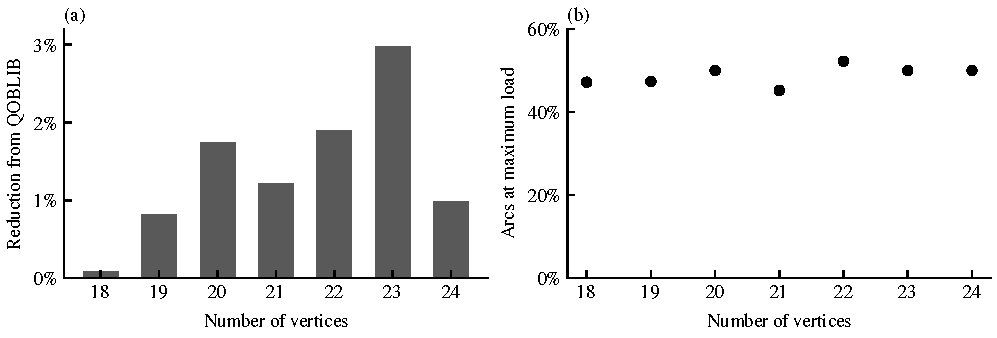
\includegraphics[width=.9\linewidth]{figures/benchmark-comparison.pdf}
\caption{First hand-in (\texttt{network18}--\texttt{network24}, before the extensions of Section 6):
(a) relative reduction in checked congestion compared with the QOBLIB reference; (b) fraction of selected arcs whose total
integer flow equals the checked objective.}
\label{fig:benchmark}
\end{figure}

Compound-move experiments on \texttt{network24} left the classical incumbent at 657,121. Across 21 QAOA rounds
with paired simulated annealing on the same QUBOs, annealing matched the logged energy in eight rounds and improved it
in thirteen. Estimating the value of QAOA on the smaller instances would require an equal-budget comparison
of the full deletion chain with a classical proposer.

The p1 trace, banked records, and replay instructions are in \path{ai_context/quantum_networks/}.
The replay starts from the archived \texttt{network24} topology. Wall-clock limits can change which candidates are explored.

\begin{thebibliography}{9}
\bibitem{hukushima1996}
K. Hukushima and K. Nemoto.
\href{https://doi.org/10.1143/JPSJ.65.1604}{Exchange Monte Carlo method and application to spin glass simulations}.
\emph{Journal of the Physical Society of Japan}, 65(6), 1604--1608, 1996.

\bibitem{lourenco}
H. R. Lourenço, O. C. Martin, and T. Stützle.
\href{https://arxiv.org/abs/math/0102188}{Iterated local search}.
In \emph{Handbook of Metaheuristics}, pp.~320--353, 2003.

\bibitem{qoblib}
QOBLIB.
\href{https://github.com/ZIB-AOPT/QOBLIB/blob/main/08-network/solutions/README.md}{Network design benchmark, best-known values}.

\bibitem{grover}
L. K. Grover.
\href{https://arxiv.org/abs/quant-ph/9605043}{A fast quantum mechanical algorithm for database search}.
In \emph{Proc. 28th ACM STOC}, pp.~212--219, 1996.

\bibitem{farhi2014}
E. Farhi, J. Goldstone, and S. Gutmann.
\href{https://arxiv.org/abs/1411.4028}{A quantum approximate optimization algorithm}.
\emph{arXiv:1411.4028}, 2014.
\end{thebibliography}

\end{document}
